%!TEX root = ../../thesis.tex

\section{Why should we temperate classifiers' predictions}
\label{chapter:limitiations:simplevsmatching}

We compare the performance of Equation~\ref{eq:matchingfilter} and Equation~\ref{eq:matchingfiltercrossvalidation} defined in chapter~\ref{chapter:lfui}. The main difference between these two equations is that the second (Equation~\ref{eq:matchingfiltercrossvalidation}) is adding another layer of verification, we temperate the prediction of the classifiers given our knowledge about their quality, which we measure by computing the confusion matrix via a cross-validation procedure.

\subsection{Artificial data}

We consider the same setting as for the experiments described in chapter~\ref{chapter:bci:EEGsignals} and used our two dimensional datasets of different qualities as presented in chapter~\ref{chapter:planning:artificialsignals}. We ran 500 simulations for each method. We consider only the planning method described in chapter~\ref{chapter:planning}.

\paragraph{Time to first task}  Figure~\ref{fig:timefirst_simplevsmatching} compares the number of iterations needed to reach the first task with confidence. We call the method using equation Equation~\ref{eq:matchingfilter} ``simple matching'' and we call ``matching'' the method using Equation~\ref{eq:matchingfiltercrossvalidation} which corrects the classifiers' predictions. There is strong differences between our method especially for low quality datasets. For extremely overlapping data (50/60\% accuracy), the ``matching'' method is never confident about a task while the ``simple matching'' method show huge variability and sometime outputs confidence after very few time steps. 

\begin{figure}[!htbp]
\centering
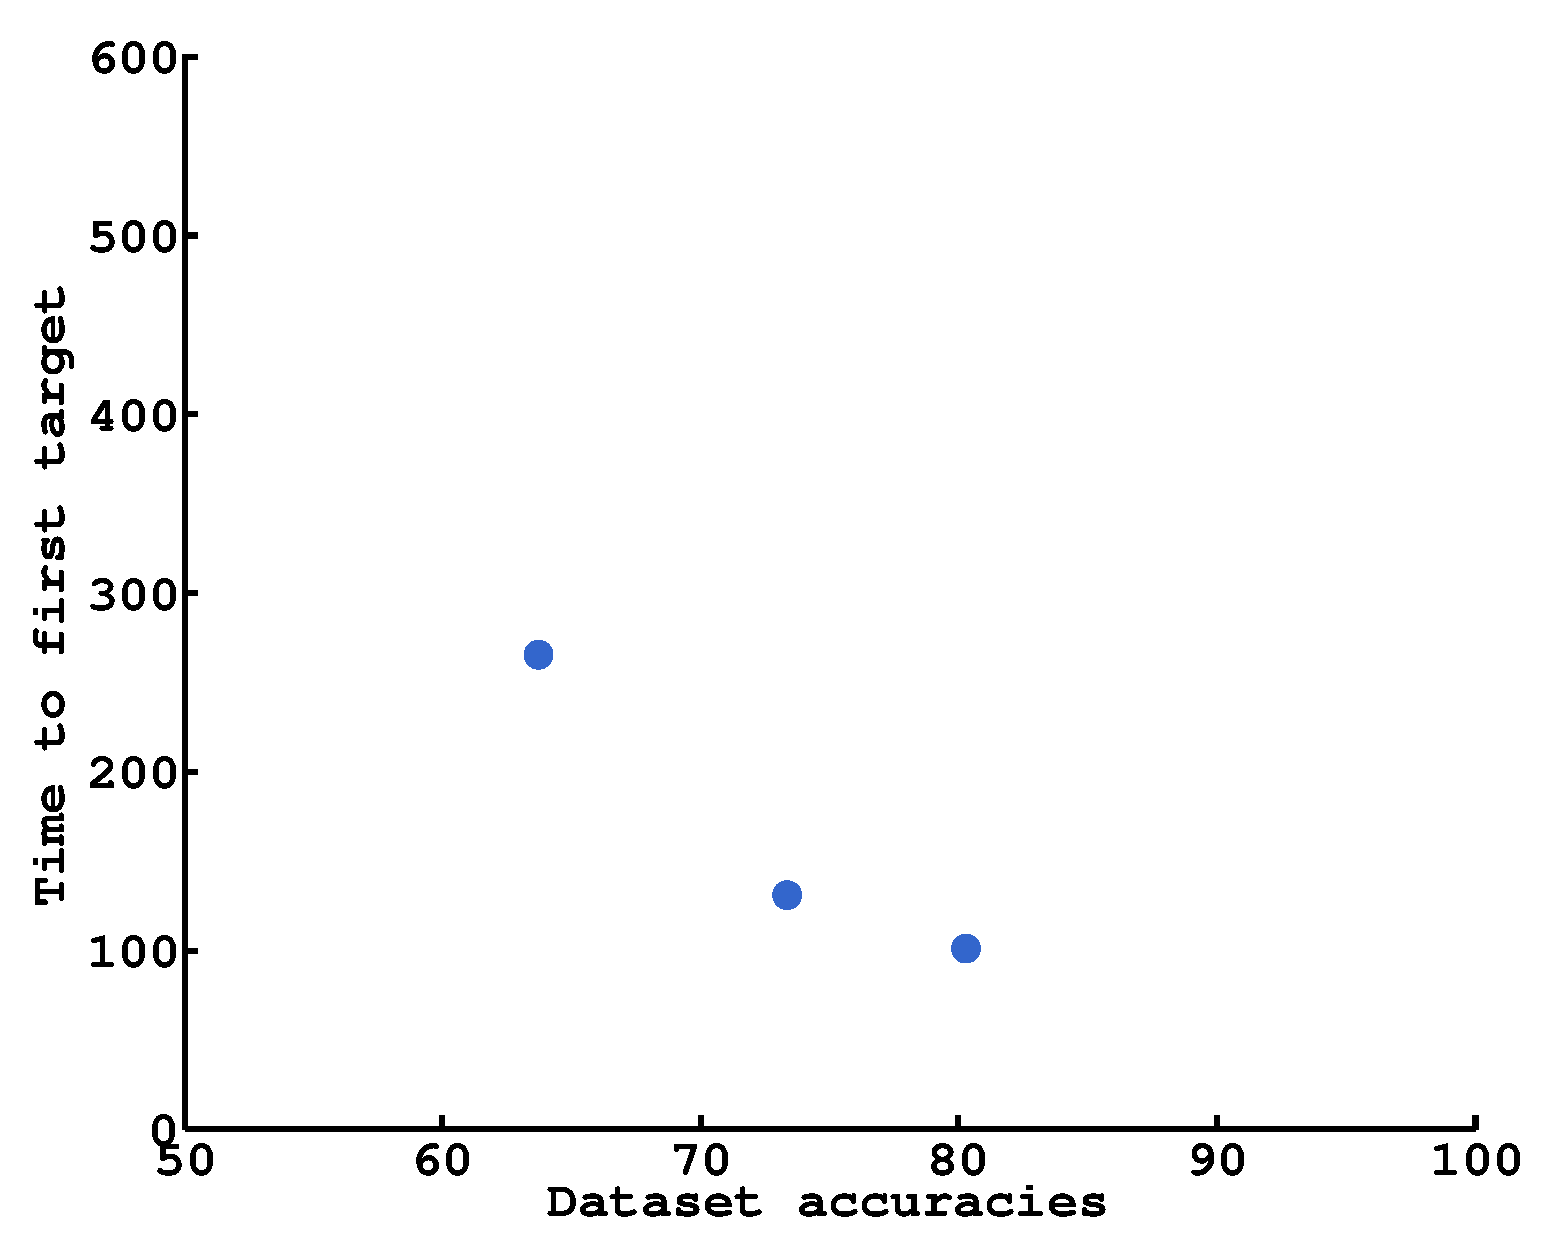
\includegraphics[width=\plotsize\columnwidth]{\imgpath/simplevsmatching/timefirst.eps}
\caption{Number of steps to complete the first task using 2D artificial datasets. Comparison between Equation~\ref{eq:matchingfilter} (simple matching) and Equation~\ref{eq:matchingfiltercrossvalidation} (matching), where the latter corrects the predictions of the classifiers given the estimation of their confusion matrix.}
\label{fig:timefirst_simplevsmatching}
\end{figure} 

This over confidence of the ``simple matching'' method reflects in the number of first tasks that were erroneously identified. As shown in Table~\ref{tab:errorTaskRatiosimplevsmatching}, the lower the quality of the data, the higher is the percentage of erroneously identified first task. For extremely overlapping data (50/60\% accuracy), this percentage go up to 20 percent. While the ``matching'' method may seems too conservative, it is particularly important to not make mistakes when estimating the first task. Indeed once a first task is identified, its associated labels are taken as ground truth. A false estimation of the first task will falsify the signal-label pairs for the remaining of the interaction.

\begin{table}[!htbp]
\centering
\rowcolors{2}{gray!25}{white}
\begin{tabular}{c c c c}
    Dataset Accuracies & Simple Matching &  Matching \\ \hline
    50-60 & 0.21 & 0 \\ 
    60-70 & 0.16 & 0 \\
    70-80 & 0.03 & 0 \\
    80-90 & 0.02 & 0 \\
    90-100 & 0.01 & 0 \\
\end{tabular}
\caption{Percentage of time the estimation of the first task was erroneous using 2D artificial datasets. Comparison between Equation~\ref{eq:matchingfilter} (simple matching) and Equation~\ref{eq:matchingfiltercrossvalidation} (matching), where the latter corrects the predictions of the classifiers given the estimation of their confusion matrix. Only the ``matching'' method, which temperates the predictions of the classifiers, does not make mistakes when estimating the first task.}
\label{tab:errorTaskRatiosimplevsmatching}
\end{table}

\paragraph{Number of tasks achieved in 500 steps}

We compare the number of tasks correctly (Figure~\ref{fig:nCorrect_simplevsmatching}) and incorrectly (Figure~\ref{fig:nWrongEEG_simplevsmatching}) achieved in 500 steps between our two methods. While the ``simple matching'' method allows to reach more targets correctly, it also makes more mistakes for low quality datasets. The ``matching'' method is more conservative and does not make mistakes for all classifier quality, at the cost of reaching less targets.

\begin{figure}[!htbp]
\centering
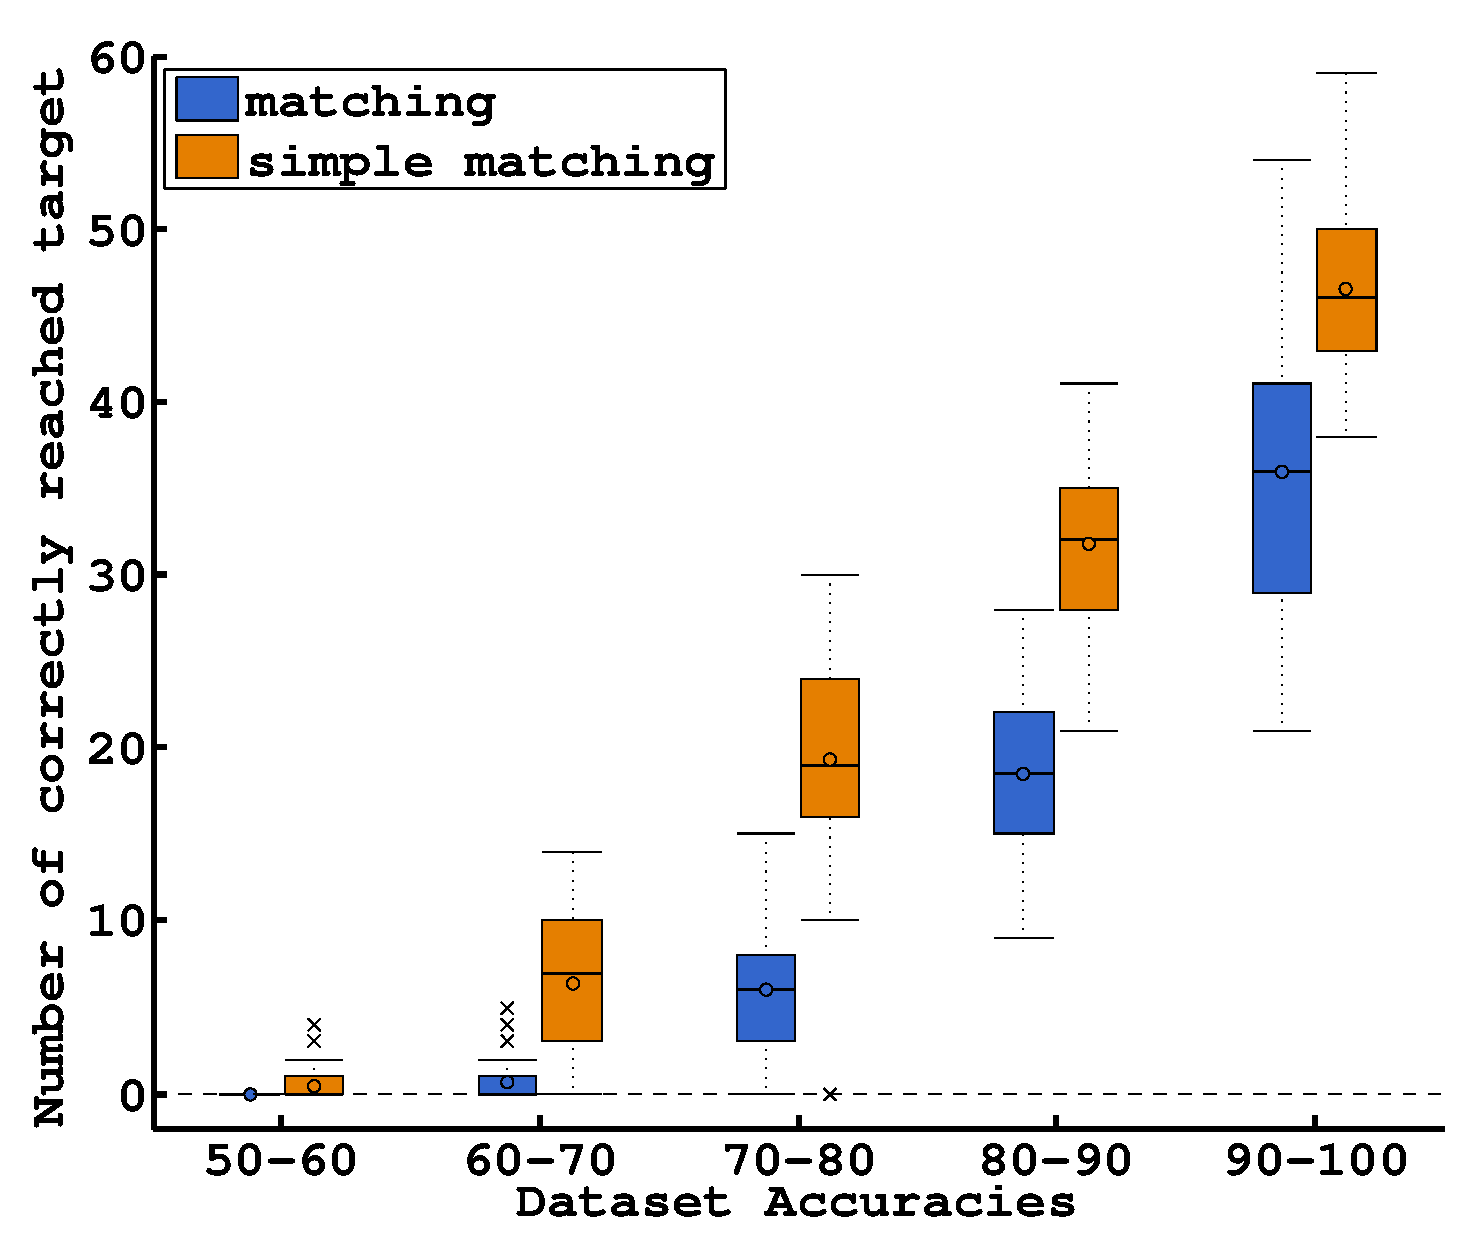
\includegraphics[width=\plotsize\columnwidth]{\imgpath/simplevsmatching/correct.eps}
\caption{Number of tasks correctly achieved in 500 steps using 2 dimensional artificial data. Comparison between Equation~\ref{eq:matchingfilter} (simple matching) and Equation~\ref{eq:matchingfiltercrossvalidation} (matching), where the latter corrects the predictions of the classifiers given the estimation of their confusion matrix. The ``simple matching'' method allows to reach more tasks correctly in 500 steps for all dataset quality.
}
\label{fig:nCorrect_simplevsmatching}
\end{figure} 

\begin{figure}[!htbp]
\centering
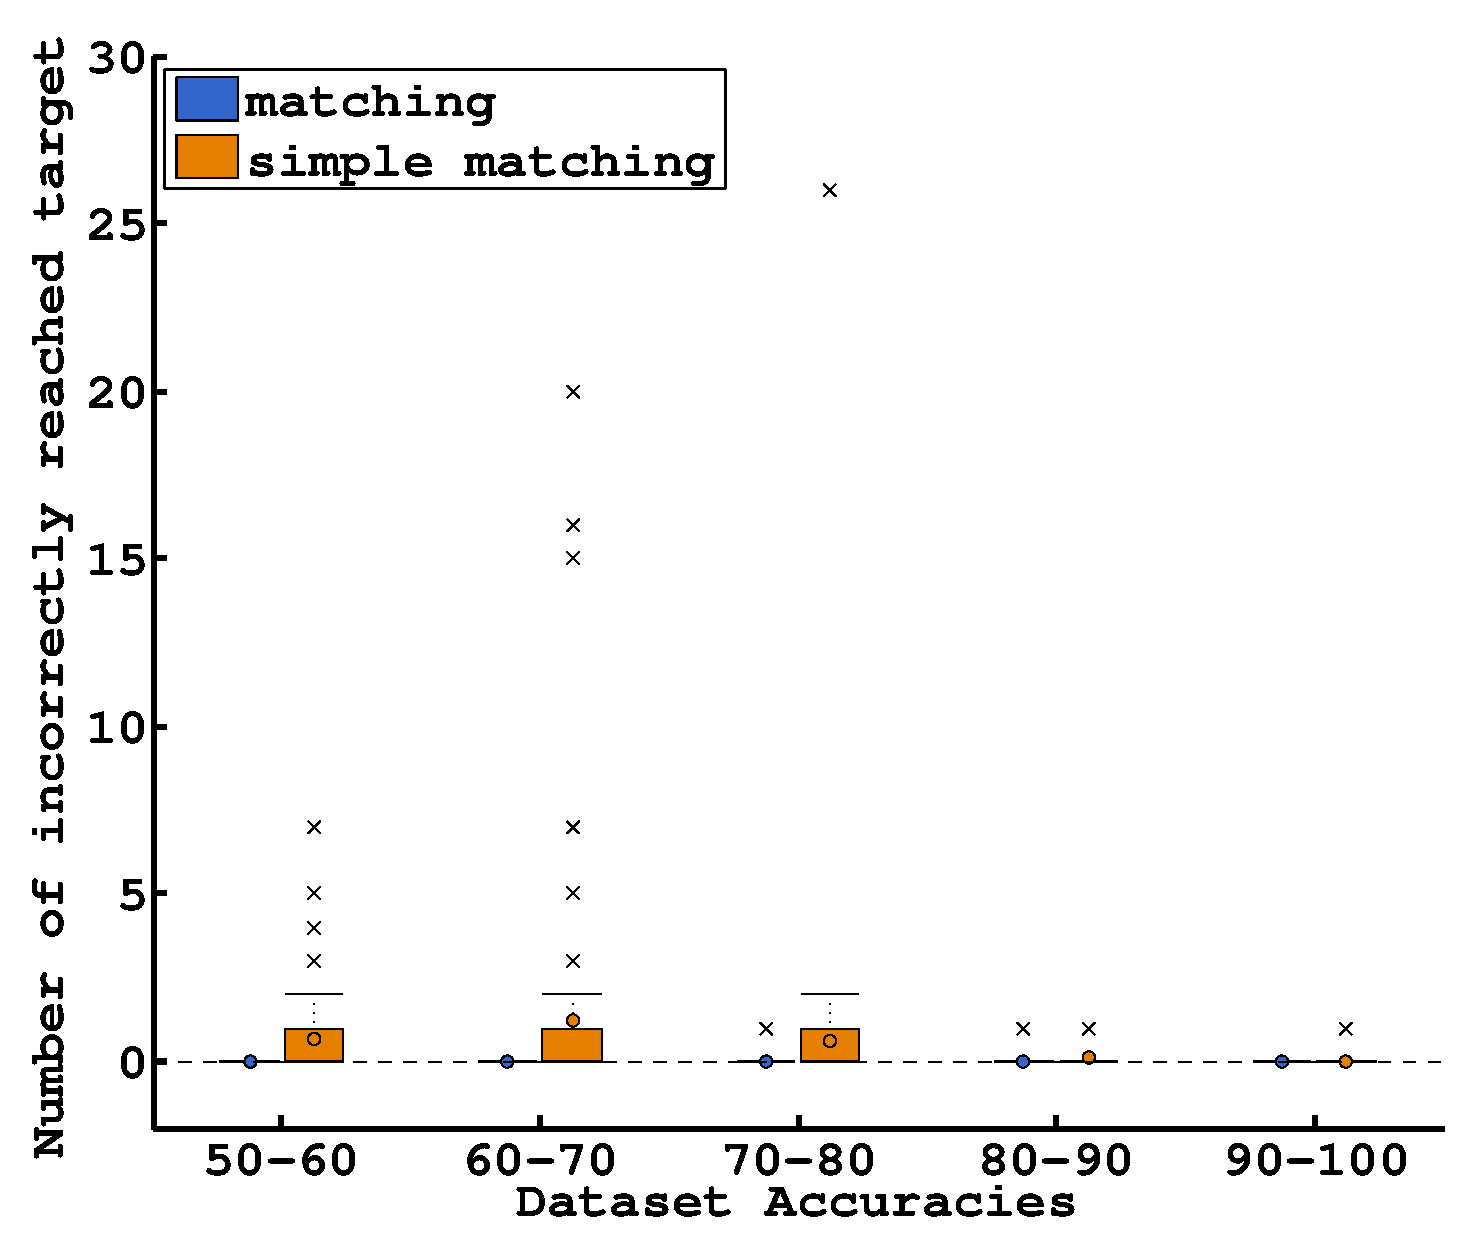
\includegraphics[width=\plotsize\columnwidth]{\imgpath/simplevsmatching/error.eps}
\caption{Number of tasks incorrectly achieved in 500 steps using 2 dimensional artificial data. Comparison between Equation~\ref{eq:matchingfilter} (simple matching) and Equation~\ref{eq:matchingfiltercrossvalidation} (matching), where the latter corrects the predictions of the classifiers given the estimation of their confusion matrix. The ``simple matching'' method starts making errors for dataset with accuracies lower than 80 percent. However, the ``matching'' method is more conservative and does not make mistakes.}
\label{fig:nWrongEEG_simplevsmatching}
\end{figure} 

\transition

These results considered only low dimensional dataset (2D), which were generated from Gaussian distribution matching perfectly with the assumption made by our classifiers. We now investigate how the performances are affected by more complex signals, such as the EEG datasets used in chapter~\ref{chapter:bci}, which are 34 dimensional with data distributions that do not necessarily follow the Gaussian assumption.

\subsection{EEG data}

We consider the same setting as for the previous subsection and use the EEG datasets described in chapter~\ref{chapter:bci}. We ran 500 simulations for each method. We consider only the active planning method used in chapter~\ref{chapter:planning}.

\paragraph{Time to first task} Figure~\ref{fig:timefirst_simplevsmatchingEEG} compares the number of iterations needed to reach the first task with confidence. There is strong differences between methods especially for low quality datasets. The ``simple matching'' method performances are not correlated with the classifiers' quality, which reflects the overconfidence of this method.

\begin{figure}[!htbp]
\centering
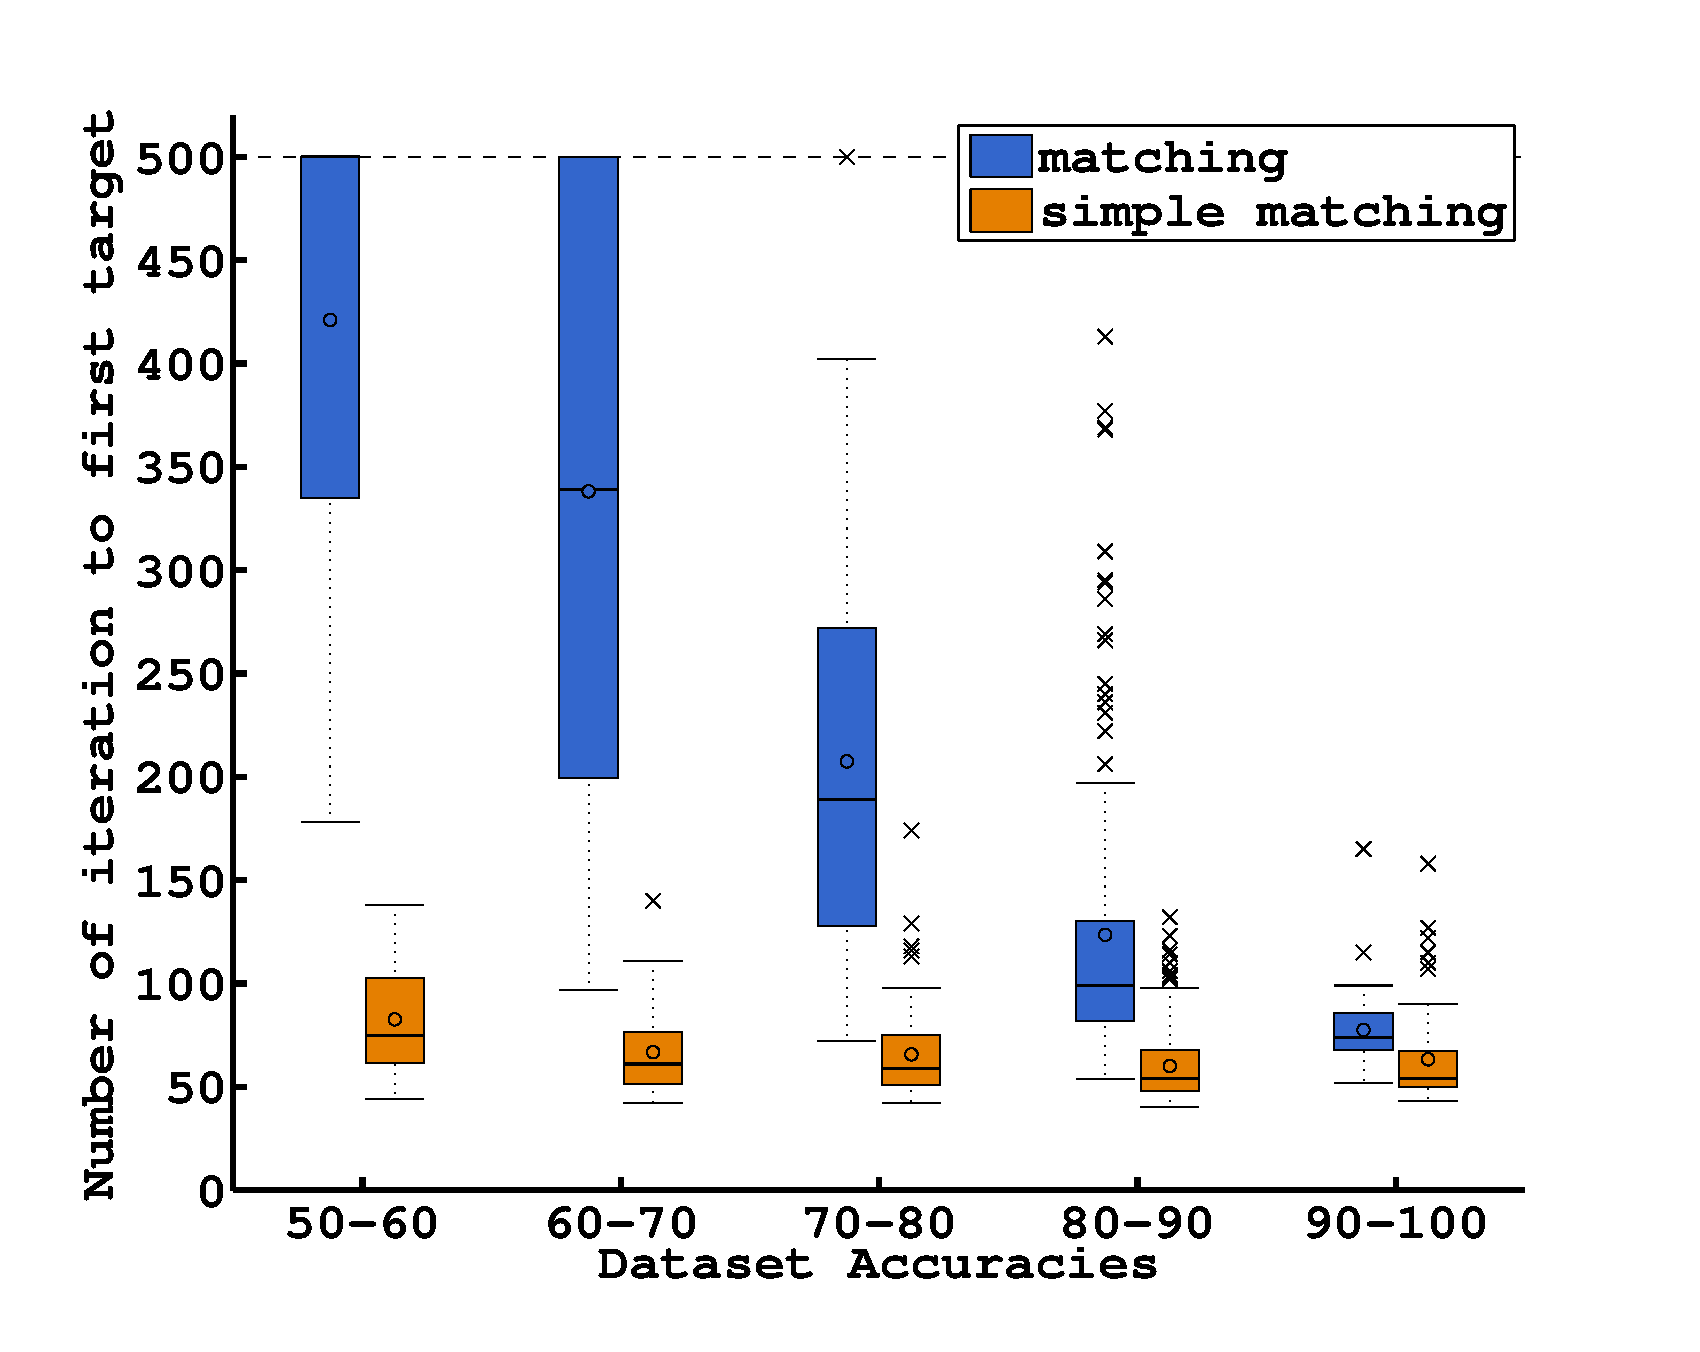
\includegraphics[width=\plotsize\columnwidth]{\imgpath/simplevsmatching/timefirstEEG.eps}
\caption{Number of steps to complete first task with our pre-recorded EEG data. Comparison between Equation~\ref{eq:matchingfilter} (simple matching) and Equation~\ref{eq:matchingfiltercrossvalidation} (matching), where the latter corrects the predictions of the classifiers given the estimation of their confusion matrix. The ``simple matching'' method performances are not correlated with the classifiers' quality, which reflects the overconfidence of this method.}
\label{fig:timefirst_simplevsmatchingEEG}
\end{figure} 

The over confidence of the ``simple matching'' method is reflected by the number of first tasks that were erroneously identified. As shown in Table~\ref{tab:errorTaskRatiosimplevsmatchingEEG}, the lower the quality of the data, the higher the percentage of erroneously identified first tasks. In all cases, this percentage was above 50 percent which makes the use of the ``simple matching'' method impossible for practical experiments. On the contrary, the ``matching'' method does not make any mistake when estimating the first task.

\begin{table}[!htbp]
\centering
\rowcolors{2}{gray!25}{white}
\begin{tabular}{c c c c}
    Dataset Accuracies & Simple Matching &  Matching \\ \hline
    50-60 & 0.81 & 0 \\ 
    60-70 & 0.80 & 0 \\
    70-80 & 0.66 & 0 \\
    80-90 & 0.53 & 0 \\
    90-100 & 0.60 & 0 \\
\end{tabular}
\caption{Percentage of time the first task estimation was erroneous using our pre-recorded EEG data. Comparison between Equation~\ref{eq:matchingfilter} (simple matching) and Equation~\ref{eq:matchingfiltercrossvalidation} (matching), where the latter corrects the predictions of the classifiers given the estimation of their confusion matrix. Only the ``matching'' method, that temperates the predictions of the classifiers does not make mistakes when estimating the first task.}
\label{tab:errorTaskRatiosimplevsmatchingEEG}
\end{table}

\paragraph{Number of tasks achieved in 500 steps}

We compare the number of task correctly (Figure~\ref{fig:nCorrect_simplevsmatchingEEG}) and incorrectly (Figure~\ref{fig:nWrongEEG_simplevsmatchingEEG}) reached in 500 steps. While the two methods allow to reach a similar number of targets correctly. The ``simple matching'' method also makes a many mistakes for all datasets. The ``matching'' method makes only few mistakes for all classifiers' quality.

\begin{figure}[!htbp]
\centering
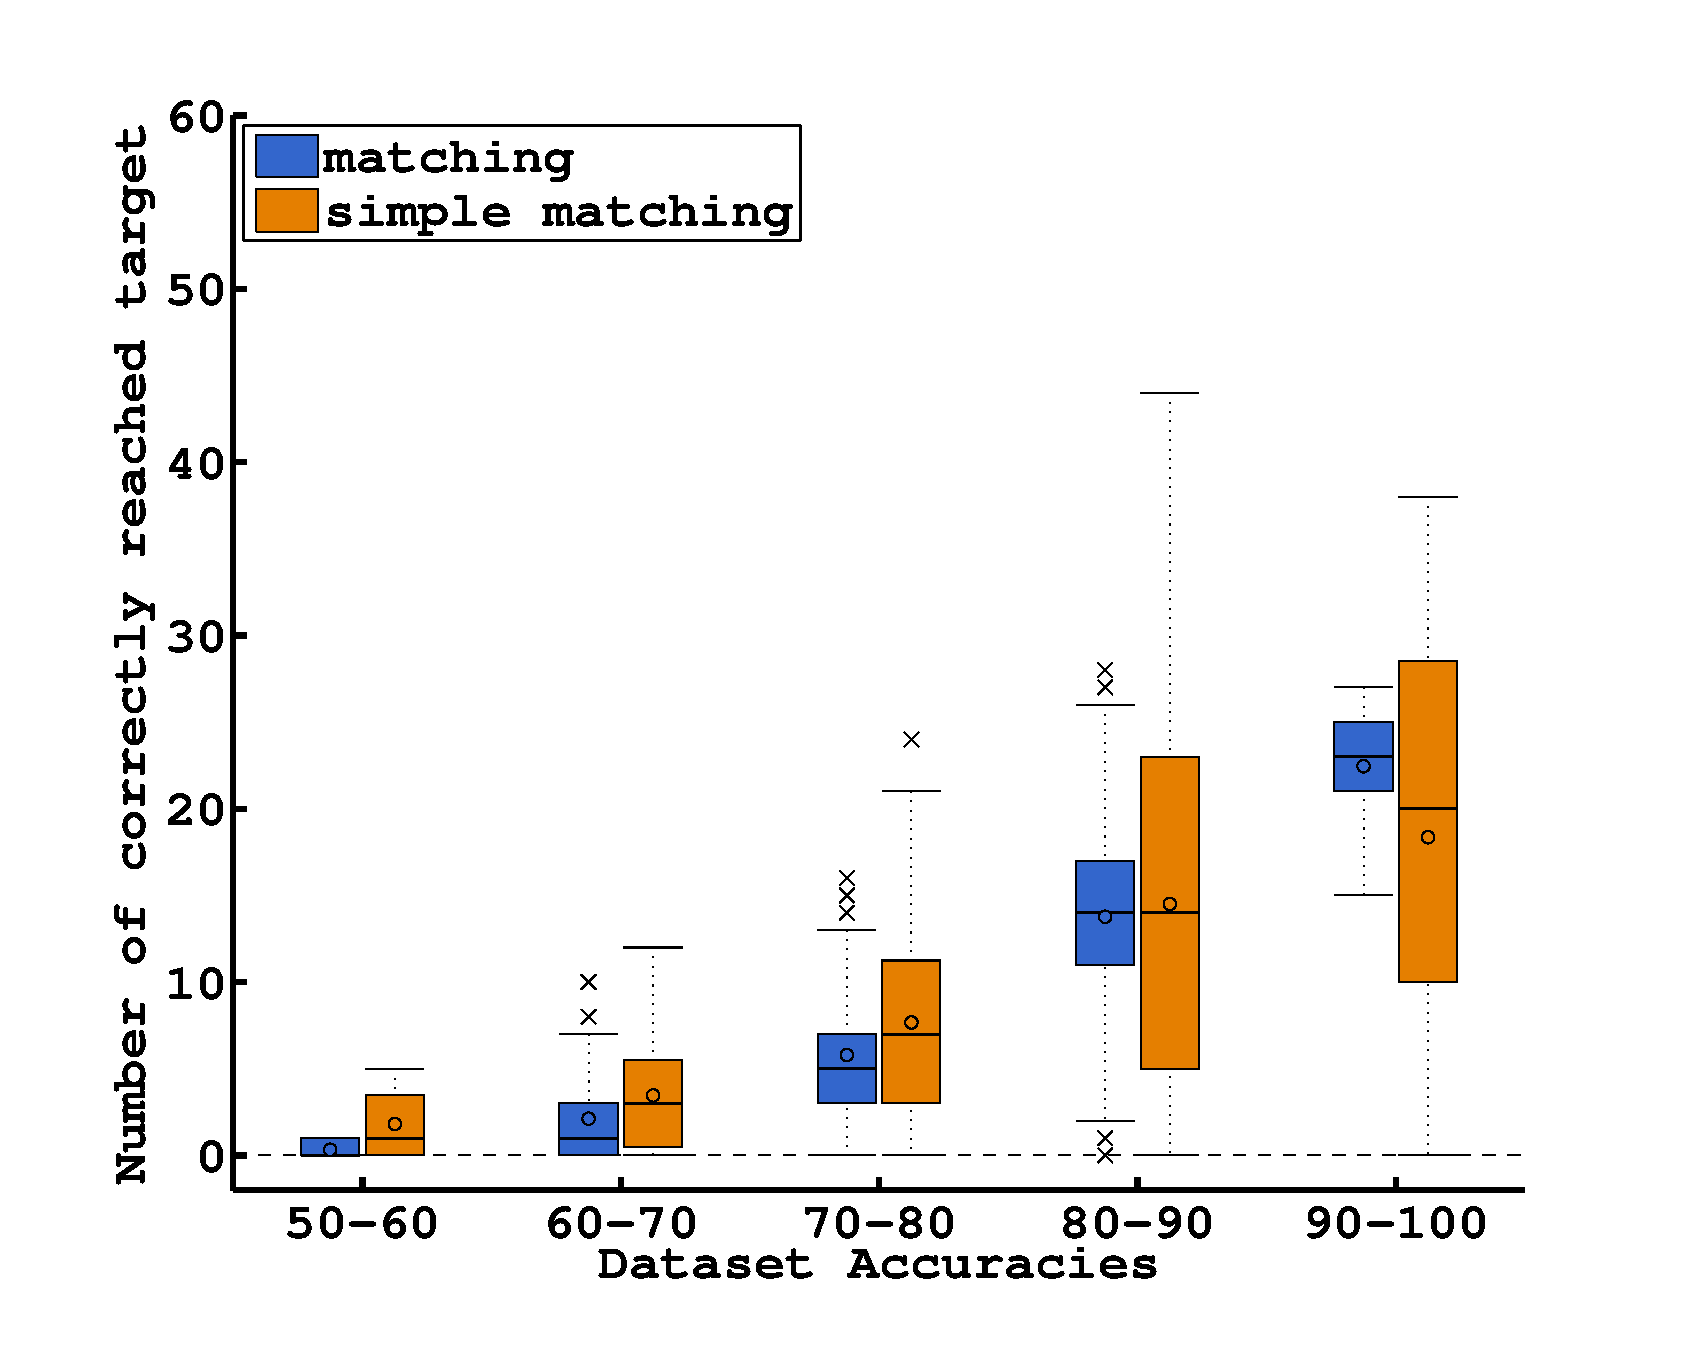
\includegraphics[width=\plotsize\columnwidth]{\imgpath/simplevsmatching/correctEEG.eps}
\caption{Number of tasks correctly achieved in 500 steps using our pre-recorded EEG data. Comparison between Equation~\ref{eq:matchingfilter} (simple matching) and Equation~\ref{eq:matchingfiltercrossvalidation} (matching), where the latter corrects the predictions of the classifiers given the estimation of their confusion matrix. Both method reach a similar number of targets correctly when using EEG datasets. The ``simple matching''  method shows more variability.}
\label{fig:nCorrect_simplevsmatchingEEG}
\end{figure} 

\begin{figure}[!htbp]
\centering
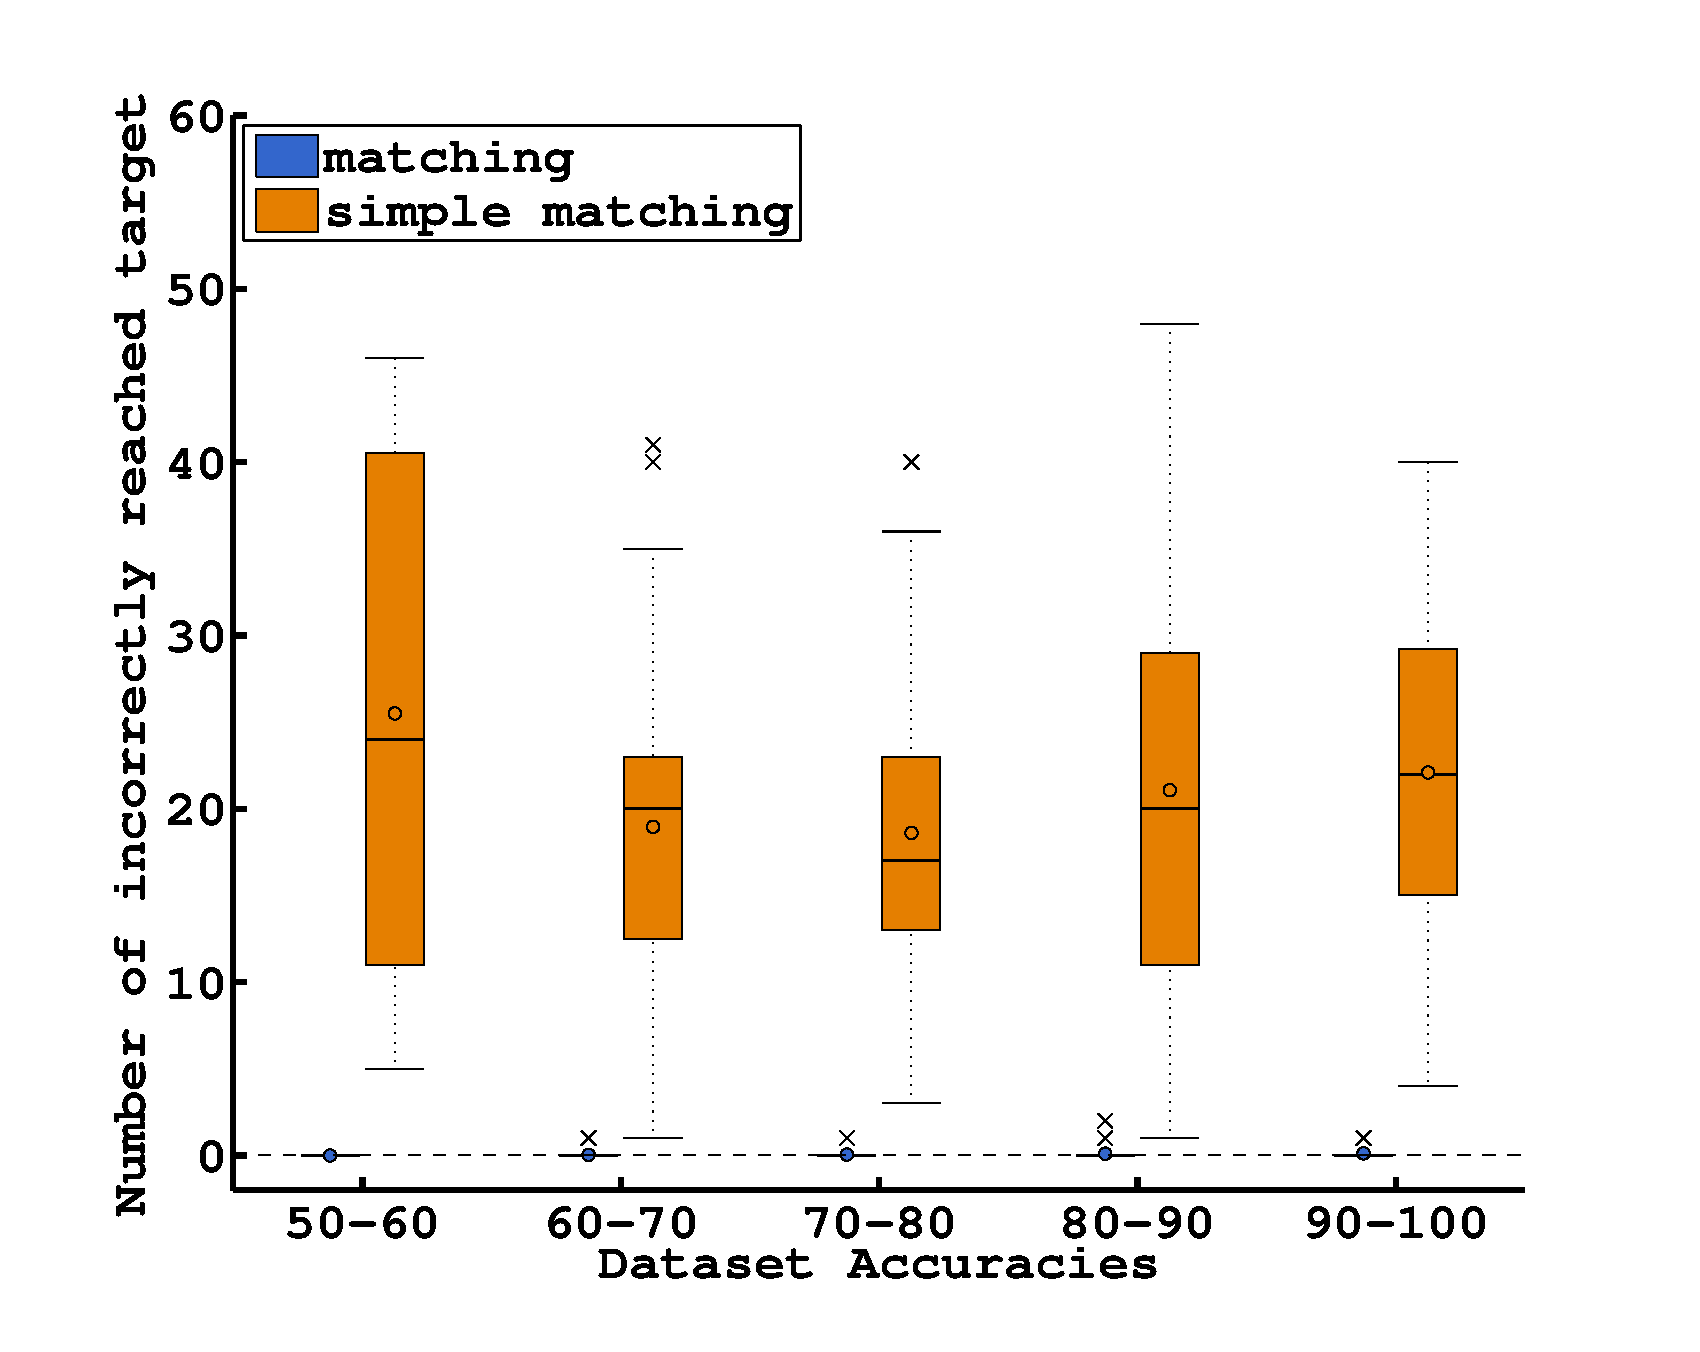
\includegraphics[width=\plotsize\columnwidth]{\imgpath/simplevsmatching/errorEEG.eps}
\caption{Number of tasks incorrectly achieved in 500 steps with our pre-recorded EEG data. Comparison between Equation~\ref{eq:matchingfilter} (simple matching) and Equation~\ref{eq:matchingfiltercrossvalidation} (matching), where the latter corrects the predictions of the classifiers given the estimation of their confusion matrix. The ``simple matching'' is not reliable for EEG data.}
\label{fig:nWrongEEG_simplevsmatchingEEG}
\end{figure} 

\subsection{Discussion}

The results presented in this section confirm that taking into account the uncertainty about the predictions of the classifiers makes the algorithm more robust. However, if we knew the data will be of good enough quality, we could afford not correcting the classifiers' outputs (as we did for the speech dataset used in chapter~\ref{chapter:lfui}), but as soon as we have to deal with a signals of various quality and with different properties (like for BCI data in chapter~\ref{chapter:bci}), it is better to include a measure of classification uncertainty in our likelihood update rule.